\section{System Design and Implementation}
\frame{\frametitle{Agenda} \tableofcontents[currentsection]}

\subsection{Design}


\begin{frame}[t]
\setbeamercovered{transparent}
\setbeamercolor{alerted text}{fg=blue}
\frametitle{Concern and solution}
\begin{columns}[T]
\begin{column}{0.5\textwidth}
  \begin{block}{\bf Design objectives}
    \begin{itemize}
        % \item<1-|alert@1> Context dependent
        % \item<3-|alert@3> Individualized
        % \item<5-|alert@5> Dynamic
        \item Context dependent
        \item Individualized
        \item Dynamic
    \end{itemize}
  \end{block}
\end{column}\hfill

\begin{column}{0.5\textwidth}
  \begin{block}{\bf What we propose}
    \begin{itemize}
        % \item<2-|alert@2> GPS location, grouped scene categories and accompanied persons
        % \item<4-|alert@4> Privacy preferences binded with facial features
        % \item<6-|alert@6> Easily update preferences, gestures (\vcenteredinclude{figure/ch4-yesgesticon.png} and \vcenteredinclude{figure/ch4-nogesticon.png}) actively speak out in capturing moment
        \item GPS location, grouped scene categories and accompanied persons
        \item Privacy preferences binded with facial features
        \item Easily update preferences, use gestures (\vcenteredinclude{figure/ch4-yesgesticon.png} and \vcenteredinclude{figure/ch4-nogesticon.png}) to actively speak out in capturing moment
    \end{itemize}
  \end{block}

\end{column}
\end{columns}
\end{frame}

\begin{frame}[t]
\frametitle{Architecture}
\begin{block}{\bf Cardea components}
  \easyfigure[0.7]{figure/ch4-cardeadesign.pdf}
\end{block}
\end{frame}

\subsection{Model Training}
\begin{frame}[t]
\setbeamercovered{transparent}
\setbeamercolor{alerted text}{fg=blue}
\frametitle{Scene classification}

\begin{columns}[T]
\begin{column}{0.3\textwidth}
  \begin{block}{\bf Training}
    \begin{itemize}
      \item<1-|alert@1-2> Dataset
      \item<3-|alert@3> Pre-trained model
      \item<4-|alert@4> Train classifier
    \end{itemize}
  \end{block}

  \only<2>{\vspace{1cm} \centering \scriptsize \color{blue} 59 categories, 10 groups, 1 million training images}
\only<3>{\vspace{1cm} \centering \scriptsize \color{blue} Place401-AlexNet}
\only<4->{\vspace{1cm} \centering \scriptsize \color{blue} {\it fc7} layer features, 60.0\% validation accuracy for scene categories, 82.8\% validation accuracy for scene groups}
\end{column}\hfill

\begin{column}{0.7\textwidth}
  \only<1>{\easyfigure{slifigure/ch4-places2.png}\vspace{-0.5cm}{\tiny Places2 dataset: \em http://places2.csail.mit.edu/index.html}\\

    \vspace{0.5cm}{\scriptsize {\color{blue} Deprecated dataset: 401 scene categories, 10 million training images}\\
Currently: 365 scene categories, 8 million training images}}

  \only<2>{

\begin{table}[tb]
\tiny
\centering
% \caption{Scene categories.}
% \label{tbl-scenecate}
\begin{tabular}{ll}
\toprule
Scene Group    & Scene Category Examples                                       \\ \midrule
Eating         & bistro/indoor, bistro/outdoor, cafeteria, coffee\_shop \\ \midrule
Entertainment  & bar, discotheque, pub/indoor                         \\ \midrule
Shopping       & bazaar/indoor, bazaar/outdoor, clothing\_store, general\_store/indoor \\ \midrule
Work           & conference\_center, conference\_room, cubicle/office, library/indoor \\ \midrule
Public         & park, street                                         \\ \midrule
Mobility       & airplane\_cabin, airport\_terminal, bus\_interior, bus\_station/indoor \\ \midrule
Exhibition     & art\_gallery, museum/indoor                          \\ \midrule
Religion       & cathedral/indoor, cathedral/outdoor, church/indoor, church/outdoor \\ \midrule
Illness        & hospital, hospital\_room, nursing\_home                \\ \midrule
Nudity         & bathroom, beach, jacuzzi/indoor, sauna, shower \\ \bottomrule
\end{tabular}
\end{table}

  }

\only<3>{\easyfigure{slifigure/ch4-placescomp.png}\vspace{-0.5cm}{\tiny\em Source: http://places2.csail.mit.edu/results2016.html}\vspace{-0.5cm}\easyfigure{slifigure/ch4-placespretrain.jpeg}\vspace{-0.5cm}{\tiny\em Source: http://github.com/metalbubble/places365}}

\only<4>{
  \vspace{-0.5cm}
  \begin{block}{\centering\bf Confusion Matrix - Category}
    \easyfigure[0.75]{figure/ch4-scnCateConfu.pdf}
  \end{block}
}

\only<5>{
  \vspace{-0.5cm}
  \begin{block}{\centering\bf Confusion Matrix - Group}
    \easyfigure[0.75]{figure/ch4-scnGrpConfu.pdf}
  \end{block}
}

\end{column}
\end{columns}


\end{frame}

\begin{frame}[t]
\frametitle{Scene classification}
\vspace{-0.5cm}
\begin{block}{\bf Prediction examples}
  \easyfigure[0.75]{figure/ch4-scnpredictemp.png}
\end{block}

\end{frame}


\begin{frame}[t]
\setbeamercovered{transparent}
\setbeamercolor{alerted text}{fg=blue}
\frametitle{Face recognition}
\vspace{-0.5cm}
\only<1-3>{\begin{columns}[T]
\begin{column}{0.5\textwidth}
\begin{block}{\bf VGG16 CNN vs Lightened CNN}
  \begin{itemize}
    \item<1-|alert@1> Model size
    \item<2-|alert@2> Feature performance
    \item<3-|alert@3> Runtime on Android
  \end{itemize}
\end{block}
\only<1>{\vspace{1cm} \centering \scriptsize \color{blue} 500MB vs 30MB}
\end{column}\hfill

\begin{column}{0.5\textwidth}
  \vspace{0.5cm}
  {\centering \tiny ({\color{blue} VGG16 CNN}) Omkar M. Parkhi et al.: \em http://www.robots.ox.ac.uk/~vgg/software/vgg\_face/}\\
  {\centering \tiny ({\color{blue} Lightened CNN}) Xiang Wu et al.: \em https://arxiv.org/abs/1511.02683}
\end{column}
\end{columns}}
\only<2>{
    \begin{figure}[!htbp]
        \centering
        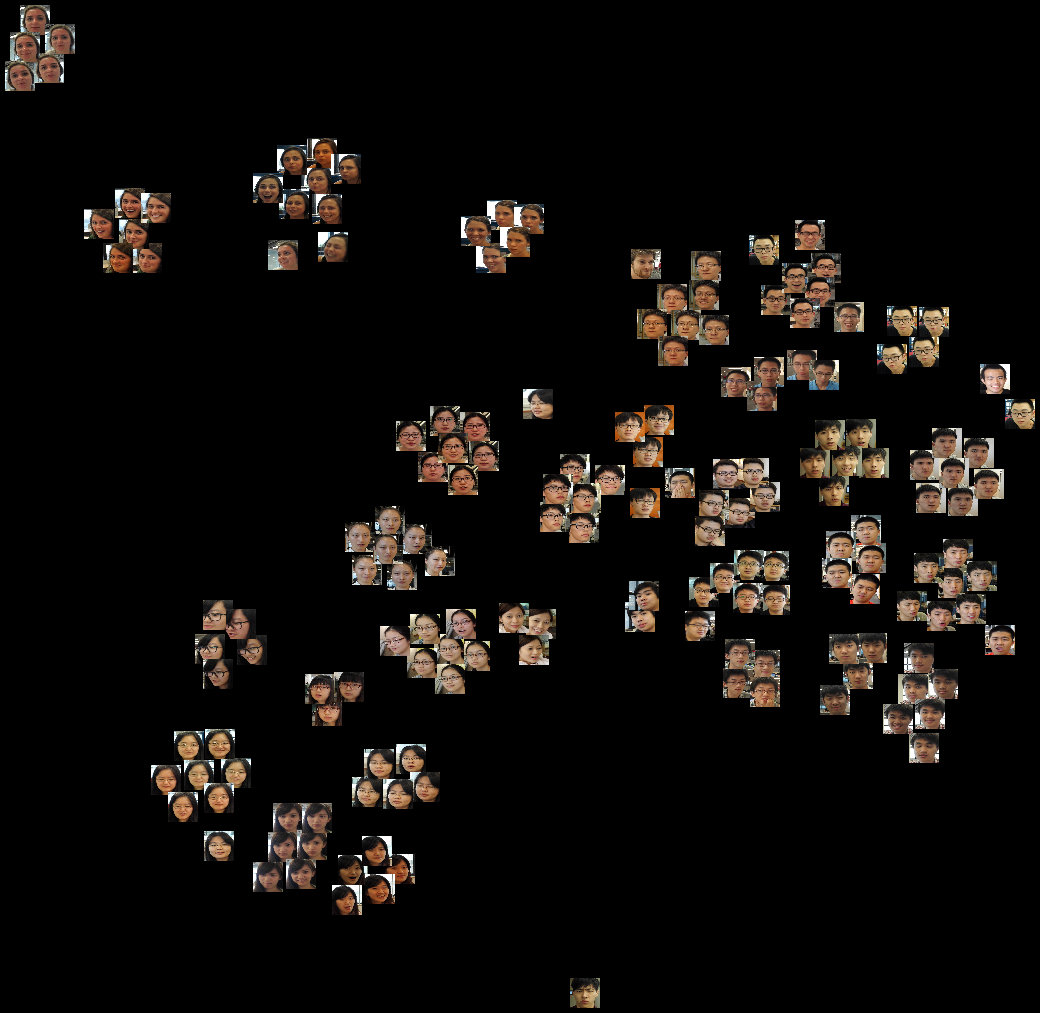
\includegraphics[height=0.5\textheight,keepaspectratio]{figure/ch4-tsnevggfc8.png}
        ~
        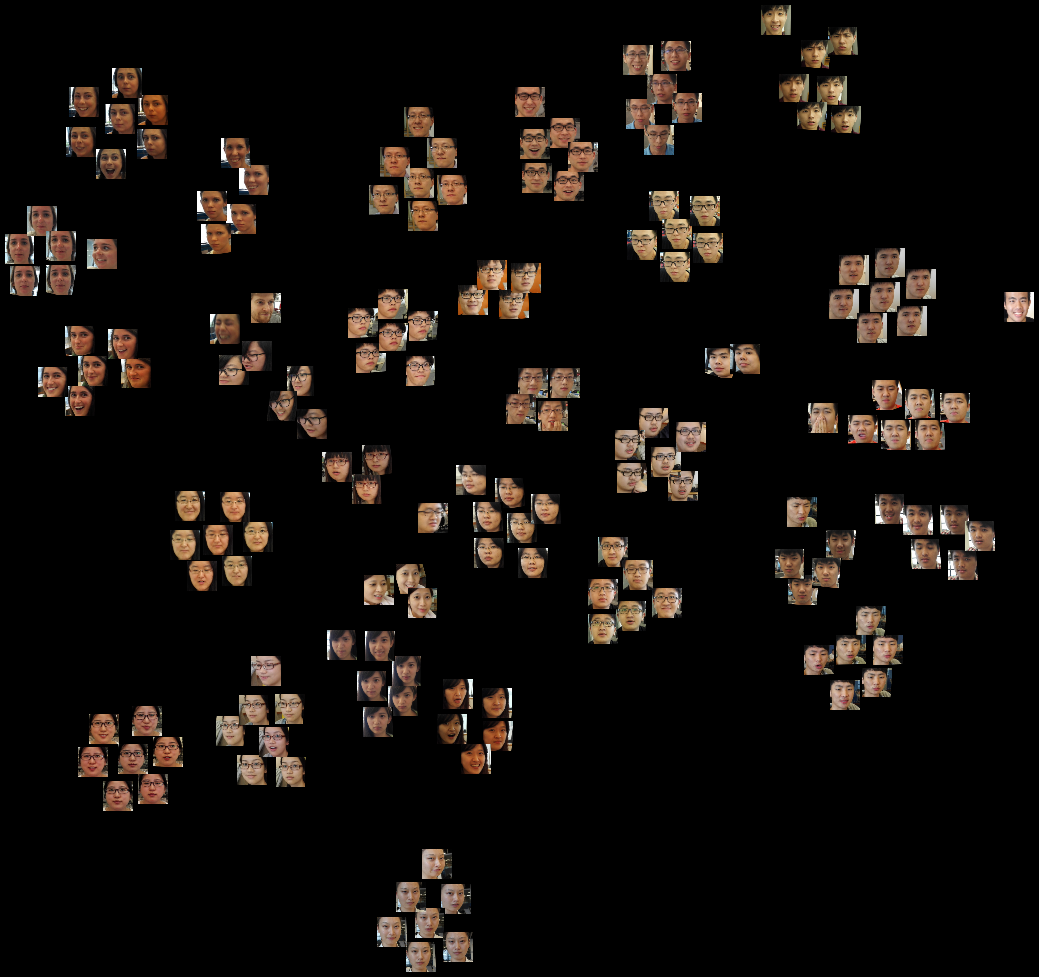
\includegraphics[height=0.5\textheight,keepaspectratio]{figure/ch4-tsnemfmeltwise_fc1.png}
    \end{figure}
}
\only<3>{

\begin{table}[!htbp]
\scriptsize
\centering
\caption{\tiny Time of single facial feature extraction and batch facial feature extraction (10 faces).}
% \label{tbl-forwardingtime}
\begin{tabular}{lrrr}
\toprule
 & Xiaomi Mi 3W & Galaxy Note 4 & Xiaomi Mi 5\\
 & {\tiny Snapdragon 800} & {\tiny Snapdragon 805} & {\tiny Snapdragon 820}\\
 & {\tiny 2GB RAM} & {\tiny 3GB RAM} & {\tiny 4GB RAM}\\
 \midrule
1 VGG CNN & N/A & N/A & $\sim 2780$ ms \\
10 VGG CNN & N/A & N/A & $\sim 26740$ ms \\
1 Lightened CNN & $\sim 508$ ms & $\sim 330$ ms & $\sim 303$ ms \\
10 Lightened CNN & $\sim 6602$ ms & $\sim 3071$ ms & $\sim 2031$ ms \\
 \bottomrule

\end{tabular}
\end{table}

}

\only<4>{
\vspace{0.5cm}
\begin{block}{\bf Detection and alignment}
  \easyfigure{figure/ch4-facedetalign.pdf}
\end{block}

\begin{block}{\bf Recognition model}
  {\centering \scriptsize \color{blue} SVM, probability threshold $T_p$ at prediction time}
\end{block}
}

\only<5>{
\vspace{0.5cm}
\begin{block}{\bf Face matching algorithm}

{\scriptsize \color{blue} Distance metric: $\mathtt{cosine}$ }

\begin{algorithm}[H]
% \caption{Face Matching}
% \label{alg:face}
\begin{algorithmic}[1] %show line numbers
\begin{scriptsize}
\STATE initialize \textit{P's} feature $f_0$, \textit{Bob's} feature $f_{i}, i \in 1, \ldots, N$, distance threshold $T_d$, hit ratio threshold $T_r$ % number of \textit{Bob's} features $N$
\STATE $m \gets 0$ $//$ number of hits
\FOR{$i=1$ to $N$}
	\STATE $d_{i} \gets dis(f_{0},f_{i})$ $//$ $dis(x,y)$ returns the distance between $x$ and $y$
	%\STATE $//$ $dis(x,y)$ returns the distance between $x$ and $y$
	\IF{$d_{i} \leq T_{d}$}
		\STATE $m \gets m + 1$
 	\ENDIF
\ENDFOR
\IF{$m / N \geq T_{r}$}
    \RETURN true $//$ \textit{P} is \textit{Bob}
\ELSE %$//$ $p \neq q$
    \RETURN false $//$ \textit{P} and \textit{Bob} are two persons
\ENDIF
\end{scriptsize}
\end{algorithmic}
\end{algorithm}


\end{block}

}

\end{frame}

\begin{frame}[t]
\setbeamercovered{transparent}
\setbeamercolor{alerted text}{fg=blue}
\frametitle{Gesture recognition}
\begin{columns}[T]
\begin{column}{0.4\textwidth}
  \begin{block}{\bf Training}
    \begin{itemize}
        \item<1-|alert@+> Dataset
        \item<2-|alert@+> Pre-trained model
        \item<3-|alert@+> Train detector
    \end{itemize}
  \end{block}

  \only<1->{\tiny\color{blue} VGG hand dataset:  5628 images with 13050 ``natural'' gesture instances, {\em \url{http://www.robots.ox.ac.uk:5000/~vgg/research/hands/index.html}}

  \vspace{0.5cm}Self prepared dataset: 4712 images with ``yes'' gestures and 3503 images with ``no'' gestures}

  \only<2->{\vspace{0.5cm} VGG16 ImageNet model}

  \only<3->{\vspace{0.5cm} Fine tune ``conv3\_1'' and up layers, approximate joint optimization}

\end{column}\hfill

\begin{column}{0.6\textwidth}
  \vspace{-0.5cm}
  \begin{block}{\centering\bf Composed dataset}
    \easyfigure[0.7]{figure/ch4-gesturedataset.png}
  \end{block}
\end{column}

\end{columns}
\end{frame}

\begin{frame}[t]
\frametitle{Gesture recognition}
\vspace{-0.5cm}
\begin{block}{\bf Prediction examples}
  \easyfigure[0.75]{figure/ch4-gestpredemp.png}
\end{block}

\end{frame}

\subsection{Integration}

\begin{frame}[t]
\frametitle{Decision flow}
\only<1>{
\begin{block}{\bf Decision path of protection action}
  \easyfigure[0.7]{figure/ch4-decisiontree.pdf}
\end{block}
}

\only<2>{
\begin{block}{\bf Example}
\begin{figure}[!htbp]
  \makebox[\textwidth]{
    \centering
    \raisebox{-0.5\height}{
      \begin{subfigure}[b]{0.55\textwidth}
        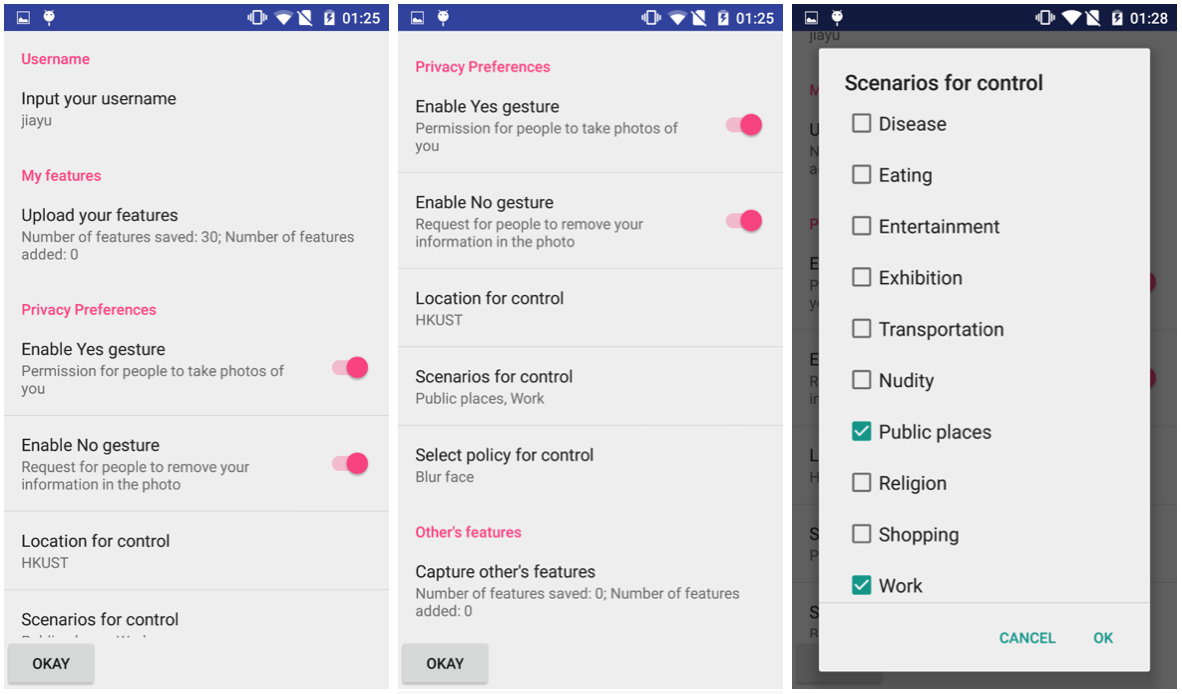
\includegraphics[width=\textwidth]{figure/ch4-reg.png}
        \caption{\scriptsize Registration and profile updating interface}
        \label{fig:ch4-reg}
      \end{subfigure}
    }
    \raisebox{-0.5\height}{
      \begin{subfigure}[b]{0.43\textwidth}
        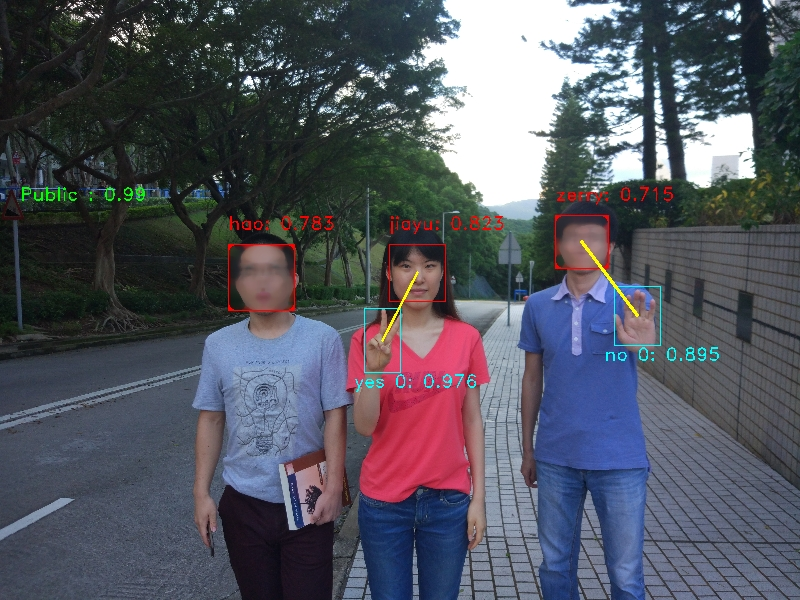
\includegraphics[width=\textwidth]{figure/ch4-allres.jpg}
        \caption{\scriptsize Privacy protection example}
        \label{fig:ch4-allres}
      \end{subfigure}
    }
  }
  \vspace{-0.25cm}
  \caption{\tiny Cardea user interface and privacy protection results. In (a), \textit{jiayu} registers as a Cardea user by extracting and uploading her face features. She specifies HKUST, two scene groups for privacy protection. She also enables ``yes'' and ``no'' gestures. In (b), a picture is taken in HKUST. 3 registered users, one ``yes'' and one ``no'' gesture are recognized. The scene is correctly predicted as ``Public''. \textit{jiayu}'s face is not blurred due to her ``yes'' gesture. Prediction probabilities are also shown in (b).}
  % \label{fig:ch4-uires}
\end{figure}
\end{block}
}

\end{frame}

\begin{frame}[t]
\frametitle{System overview}

\begin{columns}[T]
\begin{column}{0.44\textwidth}
  \begin{block}{\bf On mobile}
    \begin{itemize}
      \item face detection, alignment
      \item face feature extraction
      \item scene classification
    \end{itemize}
    {\scriptsize  OpenCV, Dlib, Caffe-android-lib}
  \end{block}
\end{column}\hfill
\begin{column}{0.5\textwidth}
  \begin{block}{\bf On cloud}
    \begin{itemize}
      \item face recognition
      \item face recognition model updating
      \item gesture recognition
    \end{itemize}
    {\scriptsize Py-faster-rcnn, LIBSVM, multiprocessing/multithreading}
  \end{block}
\end{column}
\end{columns}

\vspace{1cm}
{\scriptsize  Demo video link: \em http://bit.ly/2egw2H6}


\end{frame}


